\chapter{Conversione AD}

\begin{figure}[h]
    \centering
    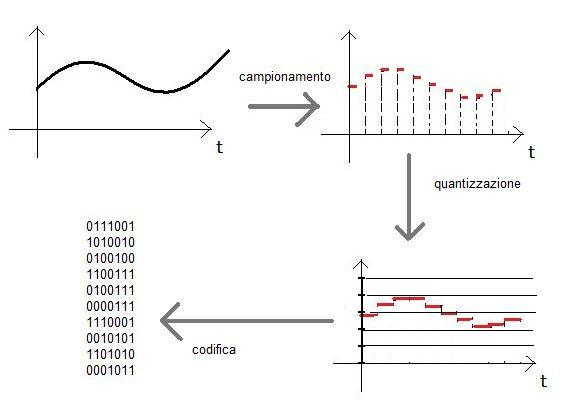
\includegraphics[scale = 1]{campdig.jpg}
\end{figure}

\newpage 

\section{Quantizzazione}
\footnote{Slide del prof | Conversione AD | pag 1.1 
}

Data una funzione analogica, cioè una funzione con infiniti valori sia nel tempo che nelle ascisse, 
la si vuole discretizzare in modo da essere reinterpretata dai circuiti digitali. \newline 

Per discretizzarla sull'asse dei tempi, alla funzione deve essere applicato il campionamento. \newline 

\begin{tcolorbox}
    Argomento ripreso da quasi tutti i corsi di ingegneria elettronica. \newline 

    Da  \url{https://github.com/ciccio25/appunti-misure-elettroniche} \\
    Capitolo 7.4 Teorema fondamentale del campionamento | pag 112 \newline 

    Per il campionamento, è stato rivoluzionario il teorema del campionamento scritto dal matematico 
    Claude. \newline 

Di seguito il teorema fondamentale del campionamento: 

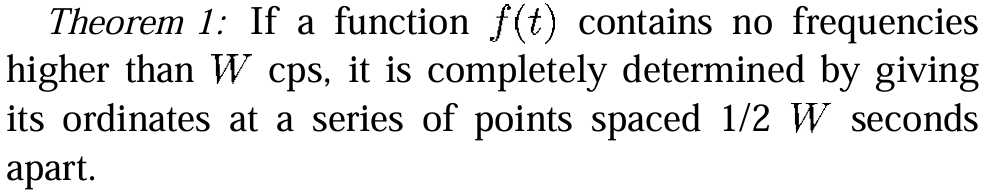
\includegraphics[scale = 0.5]{Teorema fondamentale del campionamento originale.PNG}

\begin{tcolorbox}
    Shannon pubblicò il suo teorema nella seguente rivista: 
    "Claude E. Shannon Communication in the Presence of Noise
Proceedings of the IRE, vol. 37, no. 1, pp. 10-21, Jan. 1949" 
consultabile al seguente link \\ \url{https://webusers.imj-prg.fr/~antoine.chambert-loir/enseignement/2020-21/shannon/shannon1949.pdf}
\end{tcolorbox}

Visto che il teorema è stato pubblicato nel 1949, alcune terminologie sono diverse da quello al giorno d'oggi. \newline 

Le seguenti terminologie sono: 

\begin{itemize}
    \item cps è un'abbreviazione di cycles per second, nei giorni odierni utilizziamo l'indicazione di Hz 
    \item per ordinates si intendono i valori istantanei 
\end{itemize}

La traduzione italiana, con i seguenti adattamenti, del teorema fondamentale del campionamento è la seguente: \newline 

Se la funzione f(t) contiene nessuna frequenza maggiore di W Hz, è completamente determinata dai 
suoi valori istantanei spaziati da una serie di punti spaziati di $\frac{1}{2W}$ secondi tra di loro. \newline 

Questo teorema ci dice che, se gli istanti di campionamento sono opportunamente individuati, 
la funzione che si ottiene andando a prelevare il valore istantaneo del segnale solo in quegli istanti, 
è completamente determinata, quindi non si ha perdita di informazione. \newline 

\end{tcolorbox}

Una volta che la funzione è campionata, quindi è discretizzata nell'asse dei tempi, la si può discretizzare nell'asse delle ascisse. \newline 

La discretizzazione nell'asse delle ascisse prende il nome di quantizzazione. \newline

\newpage 

Possiamo graficare i processi di discretizzazione svolti con questa figura: 

\begin{figure}[h]
    \centering
    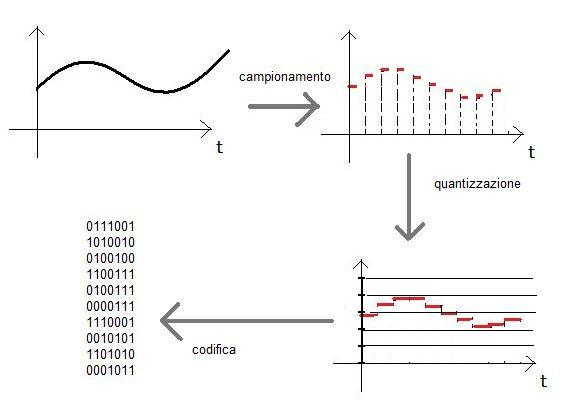
\includegraphics[scale = 1]{campdig.jpg}
\end{figure}

\begin{tcolorbox}
    Per chi come me ha svolto prima o ha seguito le lezioni del terzo anno di Misure Elettroniche della mitica prof.ssa Spinsante, 
    alcune terminologie sono differenti, ma alla fine andiamo a finire negli stessi argomenti sotto l'occhio non di un misurista, 
    bensì di un telecomunicazionista
\end{tcolorbox}

La discretizzazione può essere di due tipi, in base a come si divide l'asse delle ordinate: 

\begin{itemize}
    \item quantizzazione scalare, ogni intervallo è costante 
    \item quantizzazione non uniforme, ogni intervallo non è costante rispetto agli altri
\end{itemize}

\begin{tcolorbox}
    Per tutta la quantizzazione, rimando al corso di Misure elettroniche dove è spiegato benissimo. \newline  
    
    Da  \url{https://github.com/ciccio25/appunti-misure-elettroniche} \\
    Capitolo 7.8 Fase 2: Quantizzazione | pag 122 - 124 \newline 

    Nel corso di Misure Elettroniche, abbiamo affrontato solo la quantizzazione scalare. 
\end{tcolorbox}

\newpage 

\section{Quantizzazione scalare}
\footnote{Slide del prof | Conversione AD | pag 1.1 \\ 
Slide | Conversione AD | pag 1.1 
}


Data una funzione già campionata, possiamo applicare una quantizzazione scalare. \newline 

In questo tipo di quantizzazione, si associa un valore x a un valore $\hat{x_i}$, che a sua volta ricade in un valore nelle ordinate $a_i$. \newline 

Come si visualizza dalla seguente figura: 

\begin{figure}[h]
    \centering
    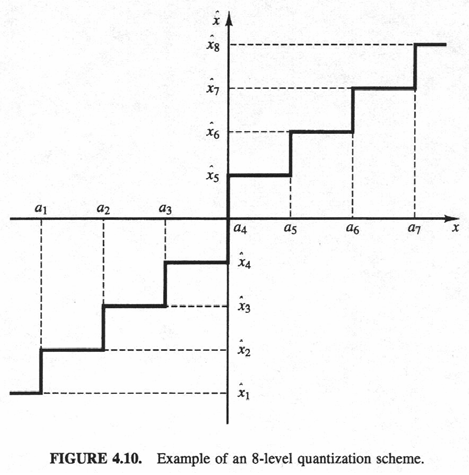
\includegraphics[scale = 1]{Quantizzazione scalare N = 8.png}
\end{figure} 

Consideriamo N il numero dei livelli di quantizzazione (in figura N = 8). \newline 

\newpage 

\subsection{Funzione di quantizzazione Q}
\footnote{Slide del prof | Conversione AD | pag 1.2 - 2.1 \\  
Slide | Conversione AD | pag 1.2 - 2.1 
}

Consideriamo Q la funzione di quantizzazione: 

{
    \Large 
    \begin{equation}
        Q(x) = \hat{x_i}
    \end{equation}
}

dove: 

\begin{itemize}
    \item x è il valore "analogico" della funzione campionata 
    \item $\hat{x_i}$ è il valore a cui è stato assegnato il valore analogico x
\end{itemize}

Per quantizzazione si intende associare un elemento sull'asse delle ascisse, 
ad un intervallo ben determinato. \newline 

La funzione di quantizzazione Q è una funzione non lineare e non invertibile, cioè, una volta svolta la quantizzazione, 
non si può ritornare al valore analogico campionato x. \newline 

In termini matematici, 
la funzione di quantizzazione Q è una funzione univoca e non biunivoca. \newline 

Lo si può spiegare meglio con il seguente grafico: 

\begin{figure}[h]
    \centering
    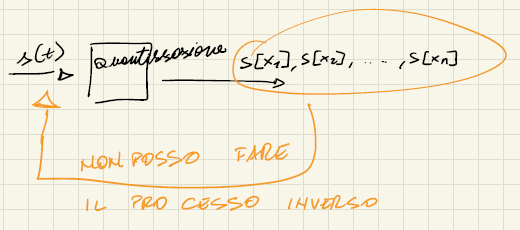
\includegraphics[scale = 0.8]{Quantizzazione funzione univoca.PNG}
\end{figure} 

Quindi, con la quantizzazione, a differenza del campionamento, parte dell'informazione viene persa nel processo di quantizzazione e non è più recuperabile. \newline 

Proprio perché nella quantizzazione Q viene assegnato un valore analogico x ad un valore discreto $x_i$, 
avviene una distorsione, e si vuole misurare quest'ultima in media quadratica. \newline 

La misura delle distorsione in media quadratica sarà: 

{
    \Large 
    \begin{equation}
            d( x, \hat{x}) 
            = 
            (x - Q(x))^{2}
            = 
            \tilde{x}^{2}
    \end{equation}
}

dove: 

\begin{itemize}
    \item $d(x, \hat{x})$ è la distanza x analogica al valore assegnato discreto $\hat{x}$
    \item $\tilde{x}^{2}$ è la media quadratica tra x e la funzione di quantizzazione Q(x)
\end{itemize}

Siccome il valore analogico x, in realtà è una variabile aleatoria, non si scrive x piccolo bensì X maiuscolo. \newline 

Quindi, riscriviamo la formula precedente dal punto di vista aleatorio: 

{
    \Large 
    \begin{equation}
        \begin{split}
          d( x, \hat{x}) 
            &= 
            (x - Q(x))^{2}
            = 
            \tilde{x}^{2} 
            \\
            &\downarrow
            \\
            D 
            &=
            \mathbb{E} 
            \left[d (X , \hat{X}) \right]^{2}
            = 
            \mathbb{E} 
            \left[ (X - Q(x) )^{2} \right] 
        \end{split}
    \end{equation}
}

in cui con il simbolo $\mathbb{E}$, dall'inglese expected value o expectation, si intende la media della variabile aleatoria contenuta nelle parentesi quadre. \newline 

\begin{tcolorbox}

    Avevamo incontrato la funzione $\mathbb{E}$ già al corso di Teoria dei Segnali. \newline 

    Da: \\
    \url{https://github.com/ciccio25/appunti-teoria-dei-segnali/blob/main/Appunti%20Teoria%20dei%20segnali.pdf} \\
    Capitolo 12.10.1 - Valore medio - pag 131 \newline 

    Per una variabile aleatoria X con densità di probabilità $f_X (x)$, il valore medio di $f_X (x)$ è fornito dal seguente integrale: 

{
    \Large 
    \begin{equation}
        m_X = \int_{- \infty}^{\infty} x \cdot f_X (x) dx
    \end{equation}
}

In alcuni casi, si indica il valore medio con la lettera, con la lettera E (dall'inglese Expectation), oppure con le parentesi $< >$: 

{
    \Large 
    \begin{equation}
        <X> = \mathbb{E}\{X\} = m_X
    \end{equation}
}

Il valore medio ha, essenzialmente, il significato di "baricentro" attorno al quale si distribuiscono i valori della variabile aleatoria X. \newline 

$\blacksquare$ \newline

Per maggiori approfondimenti: \\
\url{https://it.wikipedia.org/wiki/Valore_atteso} \newline 

    Come notazione, per quanto riguarda la statistica, si utilizzano le lettere maiuscole. \newline 

    Quindi, se x è una variabile aleatoria, non si scrive probabilità di x, bensì probabilità di X
\end{tcolorbox}

La quantizzazione scalare, a sua volta, può essere divisa in due tipi: 

\begin{itemize}
    \item quantizzazione silenziata, cioè il valore zero è un livello di quantizzazione 
    \item quantizzazione non silenziata, cioè il valore zero non è un livello di quantizzazione
\end{itemize}

\newpage 

Ritornando alla quantizzazione scalare N = 8, possiamo confrontarla con una quantizzazione silenziata: 

\begin{figure}[h]
    \centering
    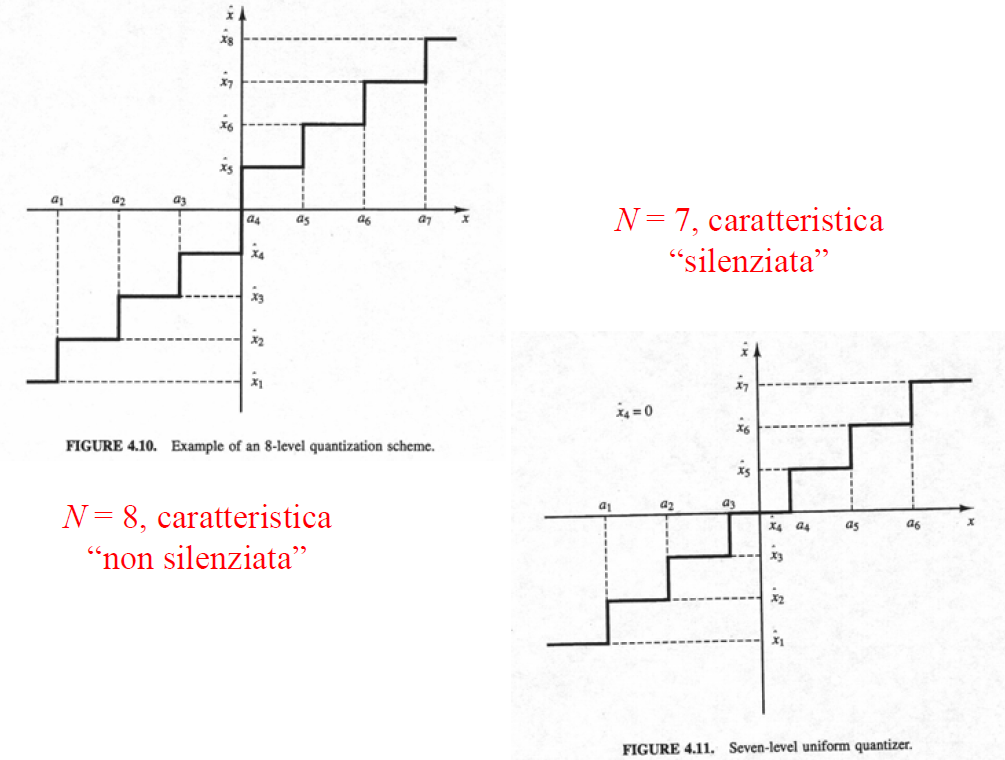
\includegraphics[scale = 0.8]{Differenza tra quantizzazione silenzata e non silenziata.PNG}
\end{figure} 

in cui si perderà un livello di quantizzazione (si passa da N = 8 a N = 7). \newline 

\newpage 

\subsubsection{Rapporto segnale-rumore di quantizzazione SQNR}
\footnote{Slide del prof | Conversione AD | pag 2.2 \\  
Slide | Conversione AD | pag 2.2 
}

Considerando il rumore come qualsiasi elemento che causa incertezza, e che quindi fa variare il valore X in un altro, 
anche la quantizzazione genera rumore. \newline 

Quindi, come nel caso dei segnali studiati nei capitoli precedenti, anche qui possiamo esprimere un rapporto segnale-rumore, 
in particolare un rapporto segnale-rumore di quantizzazione (dall'inglese SQNR Signal Quantization Noise Ratio): 

{
    \Large 
    \begin{equation}
        SQNR 
        = 
        \frac{\mathbb{E} \left[ X^{2}\right]}{\mathbb{E} \left[( X - Q(X))^{2}\right]} 
        =
        \frac{P_X}{P_{\hat{X}}}
    \end{equation}
}

dove: 

\begin{itemize}
    \item $P_X$ è la potenza del segnale utile 
    \item $P_{\hat{X}}$ è la potenza del rumore di quantizzazione
\end{itemize}

Si è potuto esprimere questa relazione perché facciamo l'ipotesi che la funzione X(t) sia stazionario. \newline 

\begin{tcolorbox}
    Queste dispense assomigliano al corso di Analisi Matematica 2, dove ogni teorema è: "Dato il teorema a una variabile studiato ad Analisi Matematica 1 $\dots$". \newline 

    Ritornando a noi. \newline 

    Per spiegare perché la potenza $P_X$ si può esprimere così, si rimanda al corso di Teoria dei segnali. \newline 
 
    Da: \\
    \url{https://github.com/ciccio25/appunti-teoria-dei-segnali/blob/main/Appunti%20Teoria%20dei%20segnali.pdf} \\
    Capitolo 13.4 - Processo ergodico e il teorema di Wiener-Khintchine - pag 156 \newline 


Nel caso di un processo ergodico, le medie di insieme (vale a dire le medie statistiche) coincidono con le medie temporali e possono essere 
calcolate a partire da un'unica e generica realizzazione del processo. \newline 

Per questo tipo di processi, possiamo enunciare il seguente teorema, il teorema di Wiener-Khintchie: 
se il processo x(t) è stazionario ed ergodico, almeno nella sua autocorrelazione, lo spettro di potenza del processo ad esso associato risulta 
la trasformata di Fourier della sua autocorrelazione statistica $R(\tau)$. \newline 


Sempre in virtù dell'ergodicità e delle proprietà ad esse associate, si può osservare che:

{
    \Large 
    \begin{equation}
        \begin{split}
            P 
            &= 
            \lim_{\Delta t \to \infty}
            \frac{1}{\Delta t}
            \int_{-\frac{\Delta t}{2}}^{\frac{\Delta t}{2}}
            x^{2} (t) dt 
            \\ 
            &= 
            \overline{R (0)}
            \\ 
            &= 
            R(0)
            \\ 
            &= 
            <x_1 ^{2}>
        \end{split}
    \end{equation}
}

\end{tcolorbox}

\newpage 

\subsection{Quantizzazione uniforme}
\footnote{Slide del prof | Conversione AD | pag 3.1 \\  
Slide | Conversione AD | pag 3.1 \\ 
Appunti | 2025-03-17 | pag 2 - 3
}

Ritornando alla figura di una quantizzazione uniforme scalare: 

\begin{figure}[h]
    \centering
    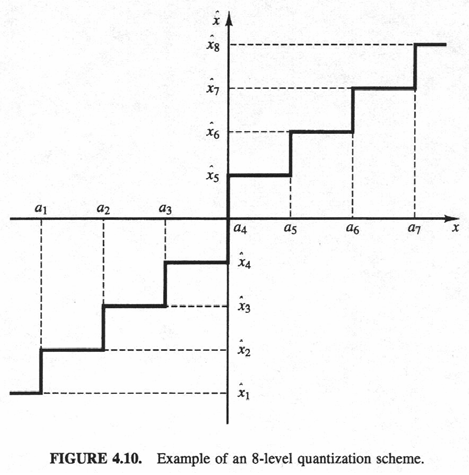
\includegraphics[scale = 1]{Quantizzazione scalare N = 8.png}
\end{figure}

L'asse reale (valori della X) è partizionato in N regioni di quantizzazione. \newline 

\begin{tcolorbox}
    Leggere il grafico è molto semplice. \newline 

    Consideriamo x un valore da quantizzare e poniamolo nell'asse delle x. \newline 

    Se x si trova in un intervallo, ad esempio si trova tra $a_1$ e $a_2$, gli viene assegnato il relativo valore di $\hat{x}$, in questo esempio $\hat{x_2}$. \newline 

    Considerando un altro esempio, x si trova tra $a_5$ e $a_6$, gli viene assegnato il valore quantizzato di $\hat{x_6}$. 
\end{tcolorbox}

Ad eccezione delle regioni $( -\infty, a_1]$ e $(a_{N-1}, + \infty)$, 
l'ampiezza di ciascuna regione è pari a $\Delta$. \newline

Quindi, dopo tutte queste considerazioni, abbiamo N + 2 gradi di libertà, cioè: 

\begin{itemize}
    \item $\hat{x_i}$ con i = 1, 2, $\dots$, N 
    \item $a_i$ 
    \item $\Delta$ l'ampiezza dell'intervallo tra le due ampiezze contigue (cioè quelle attaccate)
\end{itemize}


L'obbiettivo è quello di ottimizzare i gradi di libertà, in modo che la distorsione sia minima. \newline 

Teoricamente, per avere distorsione di quantizzazione nulla, dovremmo tendere a infinito i livelli di quantizzazione N, 
in modo tale che l'intervallo $\Delta$ tenda a zero, quindi il segnale analogico e quello quantizzato coincidono. \newline 

Ma, questo non si può fare perché, come abbiamo studiato a Teoria dei segnali, se abbiamo infiniti valori nel tempo, ciò richiederebbe infinita banda in frequenza, 
il quale non è realizzabile nei dispositivi reali. \newline 

\begin{tcolorbox}
      Da: \\
    \url{https://github.com/ciccio25/appunti-teoria-dei-segnali/blob/main/Appunti%20Teoria%20dei%20segnali.pdf} \\
    Capitolo 3.4 - Altre caratteristiche sulla dualità tempo-frequenza - pag 24 \newline 

\end{tcolorbox}

N livelli di quantizzazioni di solito non è un grado di libertà perché N ha una relazione con la banda del segnale (si spiegherà questo concetto a breve). \newline 

\newpage 

\subsubsection{Criterio a minima distanza}
\footnote{Slide del prof | Conversione AD | pag 4.1 \\  
Slide | Conversione AD | pag 4.1\\
Appunti | 2025-03-17 | pag 3 - 4
}

\begin{tcolorbox}
In questa sotto-sezione, non vi dovete ricordare le formule matematica passo passo. \newline 
Ricordatevi, piuttosto quello che scrivo per esteso, anche se è cosa buona e giusta ricordarsi le formule matematiche, specialmente all'esame orale    
\end{tcolorbox}

Ritornando all'equazione della distanza D di X con il valore quantizzato $\hat{X}$: 

{
    \Large 
    \begin{equation}
         D 
            =
            \mathbb{E} 
            \left[d (X , \hat{X}) \right]^{2}
            = 
            \mathbb{E} 
            \left[ (X - Q(x) )^{2} \right] 
    \end{equation}
}

Possiamo espandere la formula per tutti gli intervalli di quantizzazione, in questo caso in una quantizzazione uniforme. \newline 

{
    \Large
    \begin{equation}
        \begin{split}
            D 
            &=
            \mathbb{E} 
            \left[d (X , \hat{X}) \right]^{2}
            \\
            &=  
            \int_{- \infty}^{a_1}
            (x - \hat{x_1})^{2} \cdot f_X (X) dx 
            \\
            &+ 
            \int_{a_1}^{a_2}
            (x - \hat{x_2})^{2} \cdot f_X (X) dx 
            + 
            \dots
            +
            \int_{a_{N-2}}^{a_{N-1}}
            (x - \hat{x_{N-1}})^{2} \cdot f_X (X) dx 
            \\
            &+
            \int_{a_{N-1}}^{+ \infty}
            (x - \hat{x_{N}})^{2} \cdot f_X (X) dx  
            \\
            &\quad
            \\
            &=
            \int_{- \infty}^{a_1}
            (x - \hat{x_1})^{2} \cdot f_X (X) dx 
            \\
            &+ 
            \sum_{i = 1}^{N - 2}
            \left[
            \int_{a_i}^{a_{i-1}}
            (x - \hat{x_2})^{2} \cdot f_X (X) dx 
            \right]
            \\
            &+
            \int_{a_{N-1}}^{+ \infty}
            (x - \hat{x_{N}})^{2} \cdot f_X (X) dx  
        \end{split}
    \end{equation}
}

dove $f_X (x)$ è la densità di probabilità della variabile aleatoria X. \newline 

Cioè, per calcolare la distanza D tra X e i valore centrale $\hat{X}$, 
si calcola la varianza di X in ogni intervallo di quantizzazione. \newline 

Siccome il nostro obbiettivo è ottimizzare D in base all'intervallo $a_i$, 
vogliamo ci sia una distanza minima tra X e il suo valore $a_i$. \newline 

Quindi possiamo scrivere: 

{
    \Large 
    \begin{equation}
        \frac{\partial D}{\partial a_i} = 0
    \end{equation}
}

e questa relazione è valida solo se $a_i$ vale: 

{
    \Large
    \begin{equation}
        \begin{split}
            a_i 
            &= 
            \frac{\Delta}{2}
            \\
            &\quad
            \\
            &=
            \frac{\hat{x_i} + \hat{x_{i+1}}}{2}
        \end{split}
    \end{equation}
}

\begin{tcolorbox}
    Ad essere puntigliosi, in realtà, se volessimo calcolare il punto di minimo della distanza D, 
    dovremmo calcolare la derivata seconda di D su $a_i$, ma il prof a lezione ha più volte ribadito 
    che lo diamo per scontato che quel punto sia un minimo, così da fare meno calcoli matematici. \newline 

    Se vuoi farti un bel ripasso da Analisi Matematica 1 e il teorema che dimostra come calcolare i punti di massimi e di minimi in una funzione: \newline 

    Il teorema di Weierstrass, dei valori intermedi e di esistenza degli zeri - by Schooltoonchannel \\ 
    \url{https://youtu.be/k0AIKTrO7Fw?si=FNLg_2yLgPTgs6Xf}
\end{tcolorbox}


Quindi, i confini delle regioni di quantizzazione sono nel punto medio di livelli di quantizzazione adiacenti: 
ad ogni x si assegna il livello di quantizzazione più vicino. \newline 

Questo criterio prende il nome di criterio a minima distanza. \newline 

Da un punto di vista grafico, possiamo vederlo con questo esempio: 

\begin{figure}[h]
    \centering
    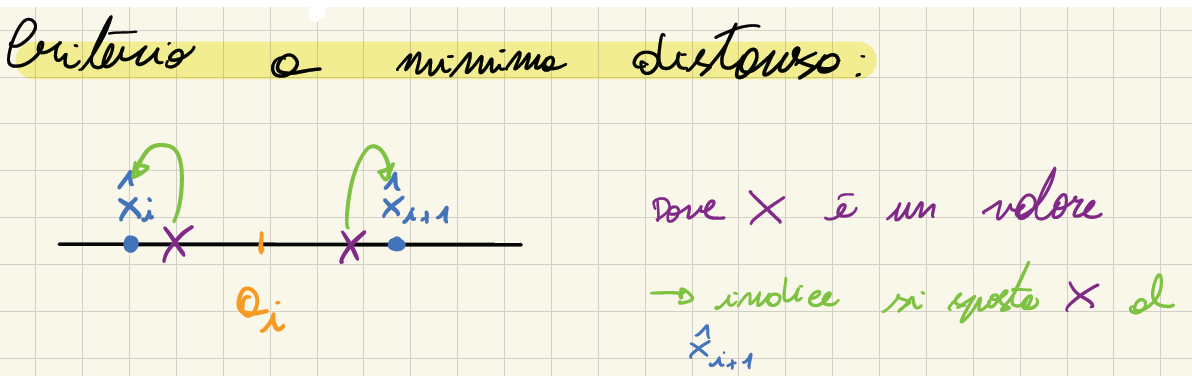
\includegraphics[scale = 0.7]{Applicazione del criterio a minima distanza.PNG}
\end{figure}

Invece se non è applicato il criterio a minima distanza, avremo questo caso: 

\begin{figure}[h]
    \centering
    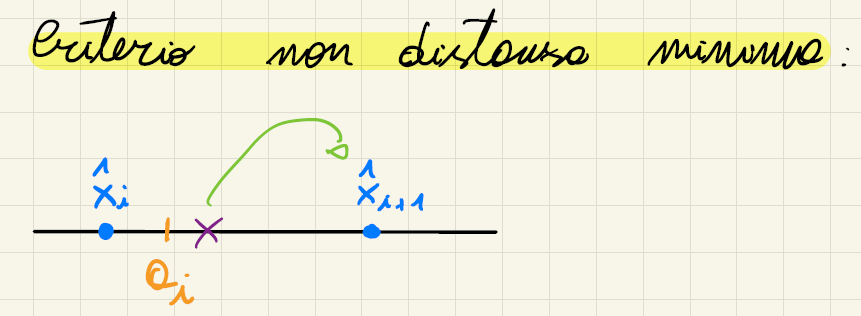
\includegraphics[scale = 0.7]{Applicazione del criterio non a minima distanza.PNG}
\end{figure}


\newpage 

\subsection{Quantizzazione non uniforme}
\footnote{Slide del prof | Conversione AD | pag 3.2\\  
Slide | Conversione AD | pag 3.2 \\
Appunti | 2025-03-17 | pag 3
}

In questo caso, rispetto alla quantizzazione uniforme, 
l'ampiezza delle regioni in cui è partizionato l'asse delle X (segnale in ingresso al quantizzatore) è variabile. \newline 

Rispetto alla quantizzazione uniforme, abbiamo 2N - 1 gradi di libertà, che sono: 

\begin{itemize}
    \item $\hat{x_i}$ in cui i = 1, 2, $\dots$, N 
    \item $a_i$ in cui i = 1, 2, $\dots$, N - 1
\end{itemize}

L'obbiettivo, anche nella quantizzazione non uniforme, è quello di ottimizzare i gradi di libertà, 
in modo che la distorsione sia minima. \newline 

Teoricamente, per avere distorsione di quantizzazione nulla, dovremmo tendere a infinito il numero dei livelli di quantizzazione N, 
in modo tale che l'intervallo $\Delta$ tenda a zero, quindi il segnale analogico e quello quantizzato coincidono. \newline 

Ma, questo non si può fare perché, come abbiamo studiato a Teoria dei segnali, se abbiamo infiniti valori nel tempo, ciò richiederebbe infinita banda in frequenza, 
il quale non è realizzabile nei dispositivi reali. \newline

\newpage 

\subsection{Ottimizzazione della quantizzazione non uniforme}
\footnote{Slide del prof | Conversione AD | pag 4.2\\  
Slide | Conversione AD | pag 4.2 \\ 
Appunti | 2025-03-17 | pag 4
}

Come il caso della quantizzazione uniforme, svolgiamo gli stessi procedimenti matematici. \newline 

Quindi dal campionatore, si avranno dei valori reali che poi saranno quantizzati. \newline 

Ritornando all'equazione della distanza D di X con il valore quantizzato $\hat{X}$: 

{
    \Large 
    \begin{equation}
         D 
            =
            \mathbb{E} 
            \left[d (X , \hat{X}) \right]^{2}
            = 
            \mathbb{E} 
            \left[ (X - Q(x) )^{2} \right] 
    \end{equation}
}

Possiamo espandere la formula per tutti gli intervalli di quantizzazione, in questo caso in una quantizzazione uniforme. \newline 

{
    \Large
    \begin{equation}
        \begin{split}
            D 
            &=
            \mathbb{E} 
            \left[d (X , \hat{X}) \right]^{2}
            \\
            &=  
            \int_{- \infty}^{a_1}
            (x - \hat{x_1})^{2} \cdot f_X (X) dx 
            \\
            &+ 
            \int_{a_1}^{a_2}
            (x - \hat{x_2})^{2} \cdot f_X (X) dx 
            + 
            \dots
            +
            \int_{a_{N-2}}^{a_{N-1}}
            (x - \hat{x_{N-1}})^{2} \cdot f_X (X) dx 
            \\
            &+
            \int_{a_{N-1}}^{+ \infty}
            (x - \hat{x_{N}})^{2} \cdot f_X (X) dx  
            \\
            &\quad
            \\
            &=
            \int_{- \infty}^{a_1}
            (x - \hat{x_1})^{2} \cdot f_X (X) dx 
            \\
            &+ 
            \sum_{i = 1}^{N - 2}
            \left[
            \int_{a_i}^{a_{i-1}}
            (x - \hat{x_2})^{2} \cdot f_X (X) dx 
            \right]
            \\
            &+
            \int_{a_{N-1}}^{+ \infty}
            (x - \hat{x_{N}})^{2} \cdot f_X (X) dx  
        \end{split}
    \end{equation}
}

dove $f_X (x)$ è la densità di probabilità della variabile aleatoria X. \newline 

Considerando la derivata di $\hat{x_i}$ sulla distanza D: 

{
    \Large 
    \begin{equation}
        \frac{\partial D}{\partial \hat{x_i}}
        =
        - \int_{a_{i-1}}^{a_i}
        2 (x - \hat{x_i}) \cdot f_X (x) dx
    \end{equation}
}

Poniamo: 

{
    \Large 
    \begin{equation}
        \frac{\partial D}{\partial \hat{x_i}}
        =
        0
    \end{equation}
}

perché vogliamo massimizzare i $\hat{x_i}$, che è un nostro grado di libertà nella quantizzazione non uniforme. \newline 

Questa relazione è vera se: 

{
    \Large 
    \begin{equation}
        \begin{split}
            \hat{x_i}
            &=
            \frac{\int_{a_{i-1}}^{a_i} x \cdot f_X (x) dx}{\int_{a_{i-1}}^{a_i} f_X (x) dx}
            \\
            &\quad
            \\
            &=
            \frac{\int_{a_{i-1}}^{a_i} x \cdot f_X (x) dx}{\Pr(a_{i-1} < X \le a_i)}
            \\
            &\quad
            \\
            &=
            \int_{a_{i-1}}^{a_i}
            \frac{ x \cdot f_X (x) dx}{\Pr(a_{i-1} < X \le a_i)}
            \\
            &\quad
            \\
            &=
            \int_{a_{i-1}}^{a_i}
            x \cdot f_X (x | a_{i-1} < X \le a_i ) dx 
            \\
            &\quad
            \\
            &= 
            \mathbb{E} \left[ x | a_{i-1} < X \le a_i \right]
        \end{split}
    \end{equation}
}

\begin{tcolorbox}
    Per gli indicatori statistici utilizzati in queste equazioni, 
    si rimanda al capitolo della probabilità studiato a Teoria dei Segnali. \newline 

      Da: \\
    \url{https://github.com/ciccio25/appunti-teoria-dei-segnali/blob/main/Appunti%20Teoria%20dei%20segnali.pdf} \\
    Capitolo 12.7 - Distribuzione di probabilità cumulativa e densità di probabilità - pag 121 - 123 \\
    Capitolo 12.13 - Densità di probabilità condizionata - pag 139  
\end{tcolorbox}

Grazie a queste formule matematiche, abbiamo dimostrato che, 
se vogliamo che $\frac{\partial D}{\partial \hat{x_i}} = 0$, 
il livello di quantizzazione della i-esimia regione corrisponde non al centro della regione, come nella quantizzazione uniforme, 
bensì al centroide di quella regione. \newline 


\newpage 

\section{Condizioni di Lloyd-Max}
\footnote{Slide del prof | Conversione AD | pag 5.1 \\  
Slide | Conversione AD | 5.1\\
Appunti | 2025-03-17 | pag 4
}

\begin{tcolorbox}
    Ho trovato una spiegazione migliore su wikipedia: \\
    \url{https://it.wikipedia.org/wiki/Algoritmo_di_Lloyd}
\end{tcolorbox}


Sapendo che: 

{
    \Large 
    \begin{equation}
        a_i = \frac{\hat{x_i} + \hat{x}_{i+1}}{2}
    \end{equation}
}

{
    \Large 
    \begin{equation}
        \hat{x_i} 
        = 
        \mathbb{E} \left[ x | a_{i-1} < X \le a_i \right] 
    \end{equation}
}

queste sono le due condizioni di Llyod-Max 
che servono per calcolare il baricentro da assegnare al quantizzatore. \newline 

È una procedura iterativa che segue questi step: 

\begin{enumerate}
    \item Si parte con un insieme (arbitrario) di regioni di quantizzazione e si calcolano gli $\hat{x_i}$ usando la seconda condizione $\hat{x_i} =  \mathbb{E} \left[ x | a_{i-1} < X \le a_i \right] $ 
    \item Si usano i livelli di quantizzazione calcolati al punto 1 per determinare nuove regioni di quantizzazione usando la prima condizione $a_i = \frac{\hat{x_i} + \hat{x}_{i+1}}{2}$
    \item Si usano le nuove regioni di quantizzazione nella seconda condizione cioè $\hat{x_i} =  \mathbb{E} \left[ x | a_{i-1} < X \le a_i \right] $ 
    \item Si ripetono alternativamente le condizioni 1, cioè $a_i$, e la seconda condizione 2, cioè $\hat{x_i}$
\end{enumerate}

\begin{tcolorbox}
    Possiamo vedere la quantizzazione scalare come una quantizzazione vettoriale con n = 1, 
    i.e. la quantizzazione scalare è una condizione particolare della quantizzazione vettoriale    
\end{tcolorbox}

\newpage 

\subsubsection{Quantizzazione uniforme e non uniforme utilizzando le tabelle}
\footnote{Slide del prof | Conversione AD | pag 5.2 - 7.1\\  
Slide | Conversione AD | pag 5.2 - 7.1\\
Appunti | 2025-03-17 | pag 4 - 6
}

Piuttosto che applicare ogni volta le condizioni di Llyod-Max, 
generalmente si utilizzano le seguenti tabelle. \newline 

Per una quantizzazione uniforme: 

\begin{figure}[h]
    \centering
    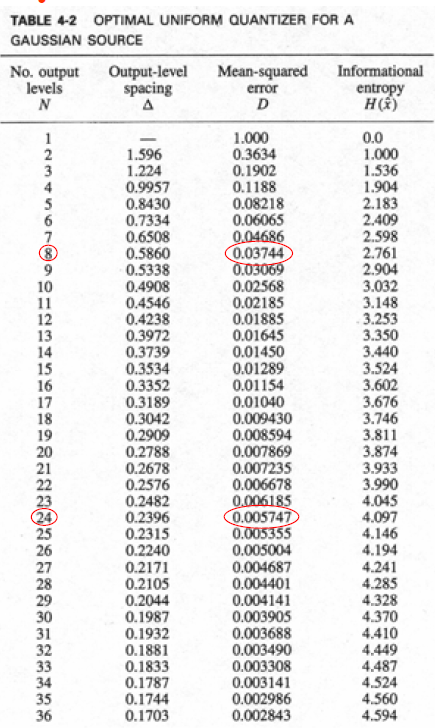
\includegraphics[scale = 0.7]{Quantizzazione uniforme tabella 1.PNG}
\end{figure}

Per una quantizzazione non uniforme: 

\begin{figure}[h]
    \centering
    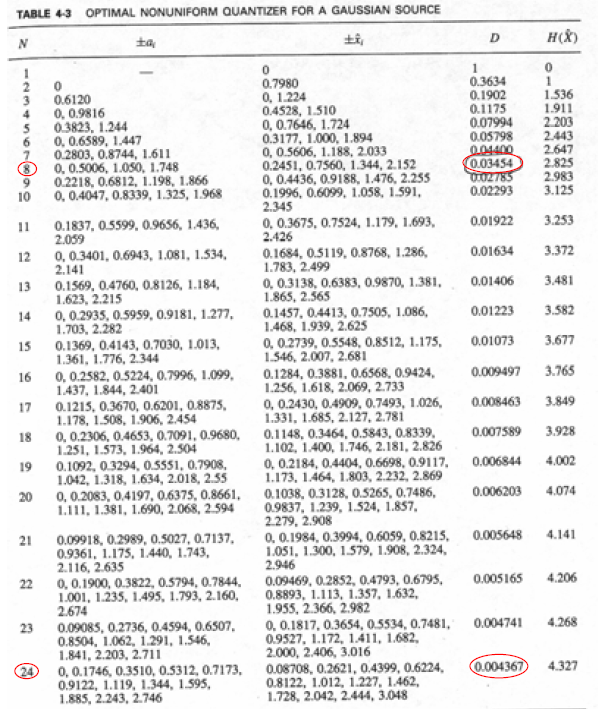
\includegraphics[scale = 0.7]{Quantizzazione non uniforme tabella 1.PNG}
\end{figure}

\newpage 

Oppure: 

\begin{figure}[h]
    \centering
    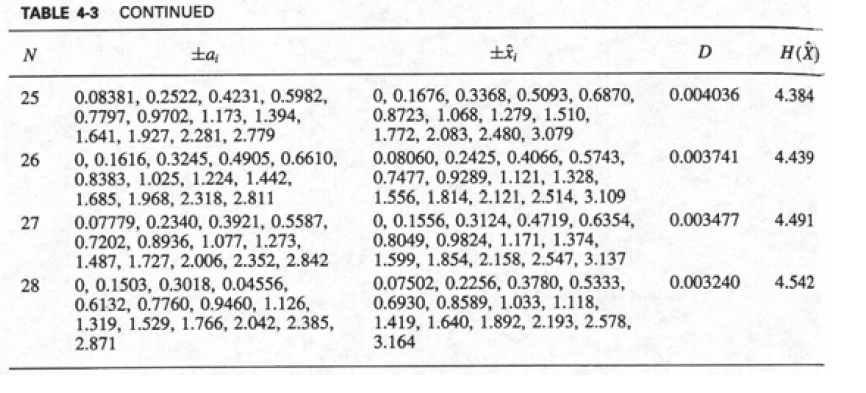
\includegraphics[scale = 0.7]{Quantizzazione non uniforme tabella 2.PNG}
\end{figure}

\newpage 

\section{Quantizzazione vettoriale}
\footnote{Slide del prof | Conversione AD | pag 7.2\\  
Slid | Conversione AD | pag 7.2\\
Appunti | 2025-03-17 | pag 6
}

Rispetto alla quantizzazione scalare in cui un campione si quantizza uno alla volta, 
nella quantizzazione vettoriale si quantizzano n campioni alla volta, dove n campione vale: 

{
    \Large 
    \begin{equation}
        n \ge 2
    \end{equation}
}

Un esempio grafico con n campioni uguale a due: 

\begin{figure}[h]
    \centering
    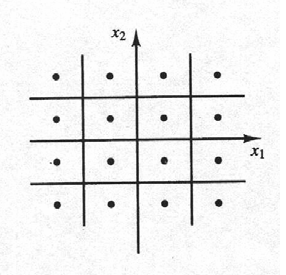
\includegraphics[scale = 1]{Quantizzazione vettoriale con n = 2.png}
\end{figure}

Come scritto nella quantizzazione scalare, anche nella quantizzazione vettoriale si hanno dei gradi di libertà, 
tra cui, come si nota dalla figura, la forma della regione. \newline 

In questo caso, ogni regione ha una forma di un parallelepipedo. \newline 

La forma della regione, generalmente, cambia in base a come il progettista del quantizzatore voglia ridurre il rumore dovuto alla quantizzazione. \newline 

Una possibile implementazione per ridurre il rumore dovuto alla quantizzazione è quella di impiegare una quantizzazione vettoriale ottima. \newline 

\newpage 

\subsection{Quantizzazione vettoriale ottima}
\footnote{Slide del prof | Conversione AD | pag 8.1\\
Slide | Conversione AD | 8.1\\  
Appunti | 2025-03-17 | pag 6 - 7
}

Nella quantizzazione vettoriale ottima, come si vede dalla seguente figura: 

\begin{figure}[h]
    \centering
    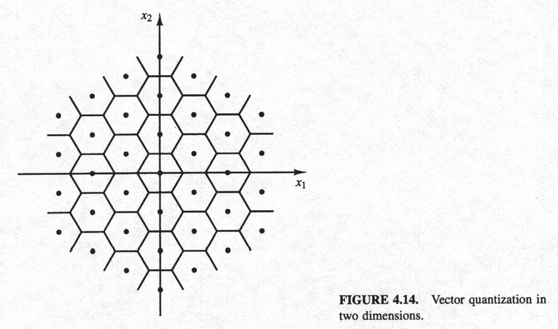
\includegraphics[scale = 1]{Quantizzatore vettoria ottima con n=2.png}
\end{figure}

si passa dalla regione rettangolare della quantizzazione vettoriale a una regione a nido d'api. \newline 

Si sceglie questa forma della regione per sottostare al teorema della distanza minima, 
cioè lo stesso studiato nella quantizzazione scalare uniforme. \newline 

Andando nello specifico della quantizzazione vettoriale ottima, 
la regione di quantizzazione i-esima è il luogo dei punti, nello spazio n dimensionale, 
che si trovano più vicini ad $\hat{x_i}$ che ad ogni altro $\hat{x_j}$ per $j \neq i$. \newline 

$\hat{x_i}$ viene definito il centroide della i-esima regione di quantizzazione. \newline 

\newpage 

\section{PCM Pulse Code Modulation}
\footnote{Slide del prof | Conversione AD | pag 8.2\\  
Slide | Conversione AD | pag 8.2\\
Appunti | 2025-03-17 | pag 7
}

La PCM è una modulazione impiegata in molti ambiti, ad esempio il canale voce negli anni 80, oppure nella lettura e scrittura dei DVD. \newline 

\begin{tcolorbox}
    Se vuoi farti una cultura: \\
    \url{https://it.wikipedia.org/wiki/Modulazione_a_impulsi_codificati}
\end{tcolorbox}

Uno schema a blocchi di una modulazione PCM è la seguente: 

\begin{figure}[h]
    \centering
    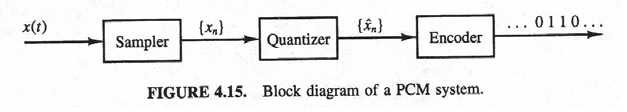
\includegraphics[scale = 1.3]{Diagramma a blocchi della PCM.png}
\end{figure}

Soffermandoci sul quantizzatore, esistono due varianti di PCM: 

\begin{itemize}
    \item PCM uniforme
    \item PCM non uniforme
\end{itemize}

\newpage 

\subsection{PCM uniforme}
\footnote{Slide del prof | Conversione AD | pag 9.1 - 10.1\\  
Slide | Conversione AD | pag 9.1 - 10.1\\
Appunti | 2025-03-17 | pag 7 
}

Facciamo le seguenti ipotesi: 

\begin{itemize}
    \item il segnale di ingresso è compreso nell'intervallo $[- x_{max}, + x_{max}]$
    \item il numero di livelli di quantizzazione è $N = 2^{v}$
    \item ciascun campione è rappresentato con v impulsi binario
\end{itemize}

Allora l'intervallo di quantizzazione $\Delta$ è:

{
    \Large 
    \begin{equation}
        \begin{split}
            \Delta 
            &= 
            \frac{\abs{- x_{max}} + \abs{x_{max}}}{N}
            \\
            &=
            \frac{2 \cdot x_{max}}{2^{v}}
            \\
            &= 
            \frac{x_{max}}{2^{v-1}}
        \end{split}
    \end{equation}
}

Ipotizzando che: 
\begin{itemize}
    \item il numero dei livelli N è molto elevato e l'intervallo di variabilità $x_{max}$ è piccolo, allora $\Delta$ sarà piccolo. \newline 
    \item il livello di quantizzazione al centro della regione di quantizzazione è al centro della regione di quantizzazione
\end{itemize}

allora l'errore è approssimabile con una distribuzione uniforme tra $-\frac{\Delta}{2}$ e $+\frac{\Delta}{2}$. \newline 

Come abbiamo con l'ottimizzazione della quantizzazione uniforme, 
calcoliamoci la potenza del segnale in PCM. \newline 

Sappiamo che $\tilde{x}$ è la differenza tra x valore analogico e Q(x) funzione di quantizzazione. \newline 

In formule: 

{
    \Large 
    \begin{equation}
        \tilde{x} = x - Q(x)
    \end{equation}
}

e questa relazione vale in tutto l'intervallo di quantizzazione, quindi in $2 \cdot x_{max}$. \newline 

Inoltre, sappiamo che $\tilde{x}$ è una variabile aleatoria nell'intervallo $\left( - \frac{\Delta}{2} , + \frac{\Delta}{2}\right]$. \newline 

Nella PCM uniforme vogliamo calcolarci la potenza di $\tilde{x}$ in ogni $\Delta$. \newline

Ricordando che, nel campionamento, consideriamo $\tilde{x}$ il rumore perché il rumore fa variare il valore campionato x, 
allora calcoliamoci la potenza del rumore, cioè la potenza di $\tilde{x}$. \newline 

Essendo $\tilde{x}$ una variabile aleatoria, allora: 

{
    \Large 
    \begin{equation}
        \begin{split}
            \mathbb{E} \left[\tilde{X }\right]^{2}
            &=
            \int_{- \frac{\Delta}{2}}^{+ \frac{\Delta}{2}}
            \frac{1}{\Delta} 
            \cdot 
            \tilde{x}^{2}
            dx
            \\
            &=
            \frac{1}{\Delta}
            \cdot 
            \left.
            \frac{\tilde{x}^{3}}{3}
            \right|_{- \frac{\Delta}{2}}^{+ \frac{\Delta}{2}}
            \\
            &= 
            \dots
            \\
            &= 
            \frac{\Delta ^{2}}{12}
            \\
            &=
            \frac{x_{max} ^{2}}{3 N^{2}}
            \\
            &= 
            \frac{x_{max} ^{2}}{3 \cdot 2^{2 v}}
            \\
            &= 
            \frac{x_{max} ^{2}}{3 \cdot 4^{v}}
        \end{split}
    \end{equation}
}


Ora che sappiamo quanto vale la potenza del rumore di quantizzazione, 
possiamo calcolarci l'SQNR (Signal to Quantization Noise Ratio): 

{
    \Large 
    \begin{equation}
        \begin{split}
            SQNR 
            &=
            \frac{\mathbb{E} [X^{2}]}{\mathbb{E} [\tilde{X}^{2}]}
            \\
            &=
            \frac{P_X}{\mathbb{E} [\tilde{X}^{2}]}
            \\
            &= 
            3 \cdot 4^{v} \cdot \frac{P_x}{x_{max} ^{2}}
            \\
            &= 
            3 \cdot 4^{v} \cdot P_{X_n}
        \end{split}
    \end{equation}
}

dove: 

\begin{itemize}
    \item $P_X$ è la potenza del segnale utile prima della quantizzazione 
    \item v sono i bit della quantizzazione 
    \item $x_{max}$ è il valore massimo che il segnale può assumere nel quantizzatore 
    \item $P_{X_n}$ è la potenza $P_X$ normalizzata, cioè $\frac{P_x}{x_{max} ^{2}}$
\end{itemize}

Molte volte può essere utile esprimere l'SQNR in dB. \newline 

Quindi la relazione di prima approssimata in dB diventa: 

{
    \Large 
    \begin{equation}
        \begin{split}
            SQNR &= 3 \cdot 4^{v} \cdot P_{X_n}
            \\
            &\downarrow
            \\
            \left.
            SQNR 
            \right|_{dB}
            &\approx
            \left.
                P_{X_n}
            \right|_{dB}
            + 
            6 \cdot v 
            +
            4.8
        \end{split}
    \end{equation}
}

Dalla formula dell'SQNR in dB si può affermare che, 
per ogni incremento di 1 nel valore di v, 
l'SQNR aumenta di 6 dB. \newline 

Anche questa osservazione ha senso da un punto di vista logico, 
perché se aumentassimo a infinito i valori di quantizzazione, il rumore di quantizzazione diminuirebbe, 
cioè l'SQNR migliora perché, in questa maniera, la quantizzazione distorce di meno il segnale di ingresso. \newline 

\newpage 

\subsection{PCM non uniforme}
\footnote{Slide del prof | Conversione AD | pag 10.2 - 12.2\\  
Slide | Conversione AD | pag 10.2 - 12.2 \\
Appunti | 2025-03-17 | pag 8
}

Al posto della PCM uniforme, quindi l'uso della quantizzazione uniforme, 
si può impiegare una PCM non uniforme, quindi l'uso della quantizzazione non uniforme. \newline 

La PCM non uniforme è molto efficace quando $f_X (x)$ differisce significativamente dall'andamento uniforme, 
cioè ci sono dei valori nella quantizzazione che sono più probabili rispetto ad altri. \newline 

Un esempio di segnale in cui i valori quantizzati sono più probabili rispetto ad altri è la voce umana 
perché i valori bassi saranno quelli più probabili rispetto a quelli alti. \newline 

Lo schema di una PCM non uniforme è la seguente: 

\begin{figure}[h]
    \centering
    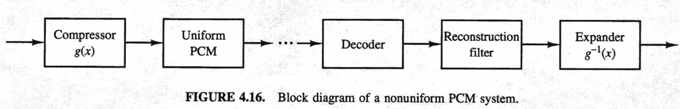
\includegraphics[scale = 1.3]{PCM non uniforme.png}
\end{figure} 

Come si nota a sinistra della figura, per rendere una PCM da uniforme a non uniforme, 
si può aggiungere prima della PCM uniforme un compressore, che ha questo tipo di andamento: 

\begin{figure}[h]
    \centering
    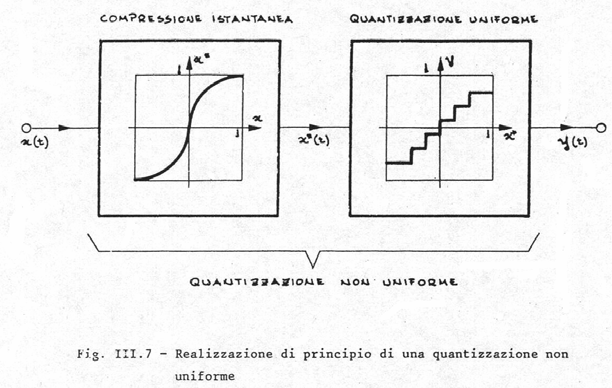
\includegraphics[scale = 0.8]{Quantizzazione non uniforme schema.png}
\end{figure} 

Per motivi storici, la legge di compressione della voce tra Stati Uniti e Europa sono diversi (ma nei nuovi standard adesso questa differenza non esiste più). \newline 

\newpage 

\subsection{Soluzioni per ridurre la banda occupata}
\footnote{Slide del prof | Conversione AD | pag 13.1 - 14.2\\  
Slide | Conversione AD | pag 13.1 - 14.2
}

Il problema più grosso della PCM è quello che, all'aumentare degli N livelli di quantizzazione, 
bisogna anche aumentare la banda del segnale modulato: 
per questo motivo, sono stati ideati e realizzati altre tecniche per diminuire la banda occupata dal segnale dopo la modulazione. \newline 

Una prima soluzione è l'uso della DPCM (Differential Pulse Code Modulation). \newline 

Nella DPCM si quantizza e si codifica la differenza tra due campioni successivi, cioè $X_n - X_{n-1}$. \newline 

Questa differenza tra i campioni successivi crea una dipendenza, in particolare una correlazione, tra i campioni. \newline 

Ma se la differenza tra i due campioni successiva è piccola, non c'è nessun problema nell'impiegare la DPCM. \newline 

Come si visualizza dal seguente schema di una DPCM: 

\begin{figure}[h]
    \centering
    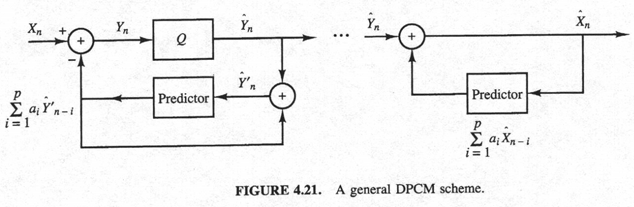
\includegraphics[scale = 1.3]{Schema DPCM.png}
\end{figure} 

si può notare il blocco del predittore (Predictor) nello schema della DPCM. \newline 

Questo perché nella DPCM il valore corrente (cioè quello di adesso) viene "predetto" sulla base di p valori quantizzati precedenti e poi si quantizza la differenza tra il valore corrente e la sua predizione. \newline 


Oppure, al posto di utilizzare una DPCM, si utilizza una modulazione Delta, 
che è un caso limite della DPCM, in cui transita solo un bit si segno (se è più grande o più piccolo di un bit rispetto al valore precedente). \newline 

\begin{figure}[h]
    \centering
    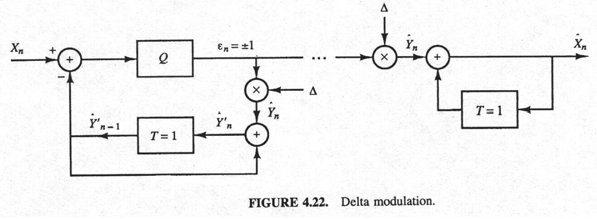
\includegraphics[scale = 1.3]{Schema modulazione delta.png}
\end{figure} 

In questo caso si utilizza una frequenza di campionamento molto elevata, 
maggiore di quella fissata dalla condizione di Nyquist. \newline 

La riduzione della banda è minore di quanto prevedibile, ma pure sempre consistente. \newline 

\newpage

Per la modulazione delta si può utilizzare anche questo tipo di architettura: 

\begin{figure}[h]
    \centering
    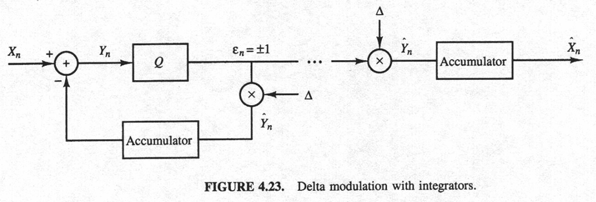
\includegraphics[scale = 1.3]{Schema modulazione delta 2.png}
\end{figure} 

\begin{tcolorbox}
    Degli ADC sigma-delta e ADC e convertitori ad inseguimento, che seguono lo stesso principio della modulazione delta 
    ne ho approfondito qui. \newline 

    \url{https://github.com/ciccio25/appunti-misure-elettroniche} \\
    Capitolo 9.8 - Convertitore ad inseguimento - pag 176 - 181 \newline

    Ma, nel caso di un telecomunicazionista, non si filtra in banda base, bensì si filtra nella banda in cui bisogna trasmettere il segnale. \newline 

    \url{https://github.com/ciccio25/appunti-misure-elettroniche} \\
    Capitolo 9.9 - Sigma-Delta $\Sigma - \Delta$ - pag 182 - 183 \newline

\end{tcolorbox}

\newpage 

